%!TEX root = main.tex
\chapter{Vorbemerkungen}

Viele der rein mathematischen Bemerkungen, Aussagen und Beispele sind Abgeleitet aus \cite{merziger2024repetitorium} und \cite{gollmann2017mathematik}. 

\section{Soundbeispiele}

Soundbeispiele sind in der Programmiersprache \texttt{FAUST} erstellt. Durch click auf das Lautsprecher Symbol sollte sich ein Browser öffnen in dem der entsprechende Klang in Echtzeit berechnet wird. Manche der Beispiele bieten Interaktionsmöglichkeit durch diverse Slider etc. Hier ein Beispiel:

\faust{Sinus, 150 Hz}{https://faustide.grame.fr/?autorun=1&voices=0&name=example&inline=aW1wb3J0KCJzdGRmYXVzdC5saWIiKTsKYW1wID0gaHNsaWRlcigiQW1wbGl0dWRlIiwgMC4yNSwgMCwgMSwgMC4wMDEpOnNpLnNtb287CnByb2Nlc3MgPSAob3Mub3NjKDE1MCkgKiBhbXApIDw6XyxfOw\%3D\%3D}

\emph{Zum Teil scheint es notwendig zu sein noch auf der großen 'RUN' Button links oben zu clicken.}

\begin{figure}[h!]
	\centering
	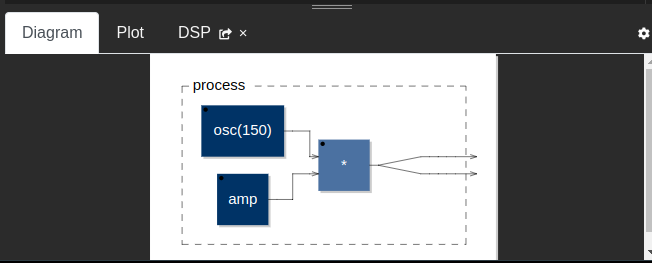
\includegraphics[width=0.8 \textwidth]{img/faust_diag.png}
	\caption{Block Diagramm in \texttt{FAUST}}
	\label{fig:faustBlock}
\end{figure}

Geneigten LeserInnen sei besonders empfohlen auch auf den 'Diagramm' button zu clicken um ein Blockdiagramm zu sehen dass dem Code/dem jeweiligen Konzept Entspricht.

\section{Python}
\todo[inline]{Formelsammlung, Griech. Alphabet.}
